\documentclass{beamer}

\mode<presentation> { \usetheme{gruvbox} }
\setbeamerfont{frametitle}{size=\huge}

\usepackage{graphicx} % Allows including images
\usepackage{booktabs} % Allows the use of \toprule, \midrule and \bottomrule in tables
%\usepackage{listings}             % Include the listings-package
\usepackage{minted}
\usepackage{tikz}
\usepackage{drawstack}
\usetikzlibrary{calc,shapes.callouts,shapes.arrows,chains,positioning,fit,shapes, arrows.meta, arrows}
\usepackage{verbatimbox}
\usepackage{tcolorbox}
\usepackage{forloop}
\usepackage{seqsplit}

\usemintedstyle{paraiso-dark}
\graphicspath{ {./images/}{../../slides-source-dep/images/} }
\DeclareGraphicsExtensions{.png,.pdf}

\newcommand{\pointthis}[2]{
    \tikz[remember picture,baseline]{\node[anchor=base,inner sep=0,outer sep=0]%
    (#1) {\underline{#1}};\node[overlay,rectangle callout,%
    callout relative pointer={(0.2cm,0.7cm)},fill=green!50] at ($(#1.north)+(-.5cm,-1.4cm)$) {#2};}%
}%

\newcounter{loopcntr}
\newcommand{\rpt}[2][1]{%
  \forloop{loopcntr}{0}{\value{loopcntr}<#1}{#2}%
}

\newcommand{\hash}[1]{{\ttfamily\seqsplit{#1}}}

\newenvironment{zerohyphen}
 {\global\chardef\savedhyphenchar=\hyphenchar\font % save the current hyphenchar
  \lefthyphenmin=1 \righthyphenmin=1 % no limits on hyphenation
  \hyphenchar\font=23 }
 {\par\hyphenchar\font=\savedhyphenchar}% eject the paragraph and restore

%----------------------------------------------------------------------------------------
%	TITLE PAGE
%----------------------------------------------------------------------------------------

\title[Introduction to Web Exploitation]{\huge \textbf{Introduction to Web Exploitation}} % The short title appears at the bottom of every slide, the full title is only on the title page

\author{Andrew Haberlandt} % Your name
\date{January 19, 2021} % Date, can be changed to a custom date

\begin{document}

{ % this brace groups the background template with just the first slide
\usebackgroundtemplate{%
    \begin{tikzpicture}
        \path [outer color = blue!5, inner color = blue!1]
        (0,0) rectangle (\paperwidth,\paperheight);
        \node[anchor=south west, inner sep=0,line width=0,draw,text width=\paperwidth,fill=almostblack] at (0,0) {\textcolor{darkgray}{\hash{00110110100011010001101101101111100010010111011001110101001111101110100101100101001000001010111000001100110000111010100100001110100010110101001010100001011100000110011111111111100110011010100100101111110111110011101011110010100001001101101010111111011000010110011101110110110000000101101101111110111010111001110010111100110110100100111110111011010110111010101101000011000100011101001011010101111101010000001000001111011111000100111001010000101010000010111001101111101111011111011001110100101101100000011000011110110111010111110001111001110011011110101001001011110001101010110000110110100011000101110110101001110100011101100111101000001001111110000111100010010110000111110101010100000000001110000001010001110110001111000100001100010110101011100011101110101100111111010111101000100111000011110110100011000110111011001101101111111100001010101010010100100101110101011111010110100111011000101010111000010110010010011000010110011000111000110110000010110001100110100011000000111100110110101011100100011110100011011010001101000110110110111110001001011101100111010100111110111010010110010100100000101011100000110011000011101010010000111010001011010100101010000101110000011001111111111110011001101010010010111111011111001110101111001010000100110110101011111101100001011001110111011011000000010110110111111011101011100111001011110011011010010011111011101101011011101010110100001100010001110100101101010111110101000000100000111101111100010011100101000010101000001011100110111110111101111101100111010010110110000001100001111011011101011111000111100111001101111010100100101111000110101011000011011010001100010111011010100111010001110110011110100000100111111000011110001001011000011111010101010000000000111000000101000111011000111100010000110001011010101110001110111010110011111101011110100010011100001111011010001100011011101100110110111111110000101010101001010010010111010101111101011010011101100010101011100001011001001001100001011001100011100011011000001011000110011010001100000011110011011010101110010001111010}}};
    \end{tikzpicture}
}


\begin{frame}
    \titlepage % Print the title page as the first slide
    \begin{tikzpicture}[overlay]
        \node[anchor=south east, yshift=-2cm, xshift=-2cm] (shirt1) at (current page.south east) {\includegraphics[width=0.15\paperwidth]{logo.png}};
    \end{tikzpicture}
    \begin{itemize}
        \item \textbf{Don't forget to start recording}
        \item Slides are on https://wiki.osucyber.club
    \end{itemize}
\end{frame}
} % end background template

\begin{frame}
    \frametitle{Opportunities this week}
    \begin{itemize}
        \item{Women in Cybersecurity Meeting, Thursday @ 7pm}
        \begin{itemize}
            \item{$<$insert topic for this week$>$}
            \item{$<$insert website/meeting link / mailing list$>$}
        \end{itemize}
        \item{Cyber Security Club Bootcamp CTF continues...}
    \end{itemize}
\end{frame}

\setbeamercolor{background canvas}{bg=almostblack}
\setbeamertemplate{section in toc}[square]
\begin{frame}
    \frametitle{Overview} % Table of contents slide, comment this block out to remove it
    \tableofcontents % Throughout your presentation, if you choose to use \section{} and \subsection{} commands, these will automatically be printed on this slide as an overview of your presentation
\end{frame}

\section{About the Bootcamp CTF}

\subsection{What is 'Capture The Flag' and why you should give it a try}

\begin{frame}
    \frametitle{What is Capture-The-Flag}
    \begin{itemize}
        \item \textbf{Essentially a hacking competition: } Each challenge contains a 'flag', which is just a secret string. For example: $ \texttt{osuctf\{th15\_15\_n0t\_a\_r34l\_flag\}} $
        \item \textbf{All of our flags are formatted like $ \texttt{osuctf\{\dots\}} $}
        \begin{itemize}
            \item \textbf{Sometimes, we'll give you a file: } You'll might have to decrypt some data, reverse engineer an executable, or analyze network traffic
            \item \textbf{Sometimes, we'll give you an IP and port: } We have set up over 20 internet-accessible services for you to hack: these include websites and APIs, as well as embedded device applications (eg. like on IoT devices)
        \end{itemize} 
    \end{itemize}
\end{frame}

\begin{frame}
    \frametitle{"CTF Scoreboard"}
    \begin{itemize}
        \item \textbf{Each challenge has an assigned point value, depending on difficulty}
        \item \textbf{Solve in any order}
    \end{itemize}
    \begin{tikzpicture}
        \node[] (shirt1) {\includegraphics[width=0.50\paperwidth]{scoreboard.png}};
    \end{tikzpicture}
    
\end{frame}

\subsection{Categories, Rules, Write-Ups, Prizes, Discord}

\begin{frame}
    \frametitle{Categories (our definitions)}
    \begin{itemize}
        \item \textbf{Web: } Vulnerabilities in web applications such as SQL injection, command injection, cross-site scripting (XSS), logic bugs, and more.
        \item \textbf{Reversing: } Figure out how a program works, without source code. (includes mobile applications, web applications, IoT firmware, ...).
        \item \textbf{Binary Exploitation: } Identifying and exploiting memory corruption and logic bugs in native executable programs. This includes some analysis of machine code and often C source code.
        \item \textbf{Crypto: } Learn about implementation flaws in encryption schemes that allow you to decrypt encrypted data sent between two parties
        \item \textbf{Forensics: } Recovering useful information from traffic captures, full disk images, a variety of common file formats (including data hidden in images). Often includes deleted / covertly recorded data.
    \end{itemize}
\end{frame}

\begin{frame}
    \frametitle{Why should you care?}
    \begin{itemize}
        \item \textbf{You want to write secure software. }Someday, you'll probably write the same kind of applications we've set up for you to hack. You'll be able to recognize a variety of vulnerabiities and avoid introducing them in your code.
        \item \textbf{Breaking other people's stuff can be fun and profitable. }Most large companies have started \textit{bug bounty} programs, which pay anywhere from \$100 - \$1,000,000 for vulnerabilites that impact the security of their systems and users.
        \begin{itemize}
            \item HackerOne and Bugcrowd are two common platforms for corporate bug bounties. Make sure you follow all the rules for any programs you participate in.
        \end{itemize}
        \item \textbf{Cybersecurity is a hot CS career field. }The skills you learn here are highly valueble to big tech, big defense, big finance, etc.
    \end{itemize}
\end{frame}

\begin{frame}
    \frametitle{About Cyber Security Club Bootcamp}
    \begin{itemize}
        \item \textbf{Bootcamp CTF: } Runs all semester. Complete challenges online.
        \item \textbf{Bootcamp Series Talks: } Will continue for... unknown period of time
        \begin{itemize}
            \item During Cyber Security Club meetings, Tuesdays @ 7pm, http://zoom.osucyber.club
            \item Talks are recorded and posted on the meeting schedule on https://wiki.osucyber.club
            \item Each talk will conclude with a list of recommended challenges
            \item \textbf{Next Week:} Intro to Cryptography
            \item Most talks are standalone, exceptions will be announced and listed on wiki
            \item Some topics will (eventually) have a 'Part 2', Web Exploitation is one of them
        \end{itemize}
        \item \textbf{How to get Started: https://go.osu.edu/CyberClubBootcamp}
    \end{itemize}
\end{frame}

\begin{frame}
    \frametitle{Rules}
    \begin{enumerate}
        \item \textbf{Don't spoil the challenges for others.}
        \begin{itemize}
            \item You are free to discuss approaches to the challenges, tools you used, important concepts, and small hints on our Discord
            \item Please do not give flags or solution guides/scripts to other participants.
        \end{itemize}
        \item \textbf{Don't try to hack the CTF scoreboard (CTFd) or the Discord. }
        \item \textbf{Be nice on the Discord.}
    \end{enumerate}
\end{frame}

\begin{frame}
    \frametitle{Prizes}
    \begin{itemize}
        \item{Prizes (while supplies last)}
        \begin{itemize}
            \item 500pts: Sticker (100 available)
            \item 2000pts: T-shirt (30 available)
        \end{itemize}
        \item{Pick up on-campus starting in Feb, or if you are remote you can wait until AU21}
    \end{itemize}
    \begin{tikzpicture}[overlay]
        \node[anchor=south east, yshift=-4cm, xshift=-2cm] (shirt1) at (current page.south east) {\includegraphics[width=0.3\paperwidth]{shirt1.png}};
        \node[left = of shirt1] (shirt2) {\includegraphics[width=0.3\paperwidth]{shirt2.png}};
        \node[anchor=north east, yshift=-4cm, xshift=-2cm] (sticker) at (current page.north east) {\includegraphics[width=0.3\paperwidth]{sticker.png}};
    \end{tikzpicture}
\end{frame}


\section{What \it{is} the 'Web' Category?}

\subsection{A little about the Internet}
\begin{frame}
    \frametitle{About the web: HTTP}
    \begin{itemize}
        \item You want to go to http://google.com \ldots How?
    \end{itemize}
    \begin{enumerate}
        \item DNS lookup for google.com $\rightarrow$ IP address
        \item Open a TCP connection, send an HTTP request message
        \item Parse HTTP response message
        \item Parse and render the HTML in the response
        \begin{itemize}
            \item Sometimes this requires additional requests for external %
            resources, which goes back to \#1
        \end{itemize}
    \end{enumerate}
   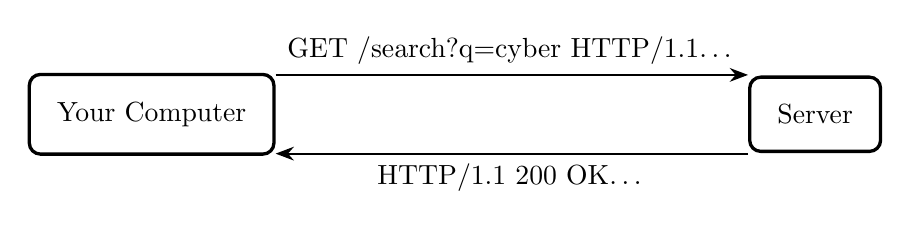
\begin{tikzpicture}[node distance=0.5cm and 3.5cm, box/.style={rectangle, rounded corners, draw, very thick, inner sep=10pt}]
	\node (computer) [box] {Your Computer};
	\node (server) [right=6cm of computer,box] {Server};
    \path [-Stealth, thick] ([yshift=0.5cm] computer.east) edge node[above] {GET /search?q=cyber HTTP/1.1\dots} ([yshift=0.5cm] server.west)
       ([yshift=-0.5cm] server.west) edge node[below] {HTTP/1.1 200 OK\dots} ([yshift=-0.5cm] computer.east);
   \end{tikzpicture}
\end{frame}


\subsection{What does a 'vulnerability' look like in a Web application?}
\begin{frame}
    \frametitle{What \it{is} the 'Web' Category?}
    Types of vulnerabilities to consider
    \begin{itemize}
        \item \textbf{Sensitive data exposure / information leakage:} Can you get %
            the server to give you information you shouldn't have access to?
        \item \textbf{Broken Access Control:} Can you modify data on the server
            without proper authorization?
        \item \textbf{Broken Authentication:} Can you login as another user or
            compromise their password or session tokens?
        \item \textbf{Manipulating Responses to other users:} Can you modify
            resources provided to other users in a way that will directly
            or indirectly give you access to their account?
    \end{itemize}
\end{frame}

\subsection{Why do we care about Web?}
\begin{frame}
    \frametitle{Why do we care?}
    \begin{itemize}
        \item There are lots of websites, with lots of data
        \item APIs
        \item Web technologies bleeding into desktop apps (Electron)
        \item Bug bounties are largely web applications (e.g. HackerOne, Bugcrowd)
    \end{itemize}
\end{frame}

\section{Demo: Using Chrome 'Developer Tools' to Hack Stuff}
\begin{frame}
    \frametitle{Demo: Chrome Developer Tools} 
\end{frame}

\subsection{HTML \& Inspect Element}
\subsection{Javascript \& the Console}
\subsection{Note about Frameworks}
\subsection{The Debugger}
\subsection{The 'Network' Tab}
\subsection{Storage}

\section{Useful Tools and What They Do}
\begin{frame}
    \frametitle{Tools}
\end{frame}

\end{document}
